\newcommand{\si}[2]{$\mathrm{#1\,#2}$}
\subsection*{Experimental setup}
\begin{figure}[ht]
	\centering
	\includegraphics{figures/experimentalSetup.png}
	\caption{Diagram of the photoluminescence spectroscopy setup.}
	\label{fig:experimentalSetup}
\end{figure}

\ref{fig:experimentalSetup} illustrates our experimental setup which we use to acquire the photoluminescence spectra. 
The beam path to excite the sample and induce photoluminescence emission is highlighted in blue.
For the excitation, we use a beam with a central wavelength of \si{405}{nm}.
This is achieved by using a laser that generates a beam with a central wavelength of \si{402}{nm} and a excitation filter to select our wavelength.
A dichroic mirror directs the beam to a lens that focusses the beam on the sample's surface.
The beam path of the emitted photoluminescence light is highlighted in red.
Starting from the sample's surface, the emitted light is collected and collimated by the lens and passes through the dichroic mirror.
To ensure that the excitation beam is completely removed from the emission path we use a longpass filter with a cut-on wavelength of \si{420}{nm}.
Once filtered, the beam passes through a lens that focusses the light onto an optical fibre which directs the light to a spectrometer (LR2, Lasertack GmbH).

Both the laser and the spectrometer are controlled with a microcontroller which, in turn, is connected to a pc.
This arrangement makes it possible to control the laser power, illumination time and the delay time to start acquiring the spectrum.
The latter is set to \si{500}{ms}.
\subsection*{Samples and measurement parameters}
\begin{table}[ht]
	\centering
	\begin{tabular}{*6l}
		\hline
		Sample Type & Number of Samples & \multicolumn{2}{c}{Measurement 1} & \multicolumn{2}{c}{Measurement 2}\\
		{}& {} & Laser Power [mW] & Illumination Time [ms] & Laser Power [mW] & Illumination Time [ms]\\
		\hline
		Non-plastic & 12 & 0.5\textendash130 & 300 & 0.2\textendash2.8 & \\
		\hline
		Plastic (manufacturer) & 26 & 5\textendash130 & 300 & 0.5\textendash100 & 300\\
		\hline
		Plastic (retail) & 8 & 0.5\textendash130 & 300\textendash1500 & 0.5\textendash104 & 300\\
		\hline
	\end{tabular}
	\caption{\label{tab:samples}Legend (350 words max). Example legend text.}
\end{table}
Our spectral data set consists of 46 samples which contains non-plastic samples from the riverine and marine environment and plastics from manufacturers and retail products.
\ref{tab:samples} gives a summary of all samples with the range of the measurement parameters used in this study.
For each sample, we acquire multiple spectra with two sets of parameters, namely laser power and illumination time.
Furthermore, the difference between the measurements are adjustments of the optical setup.
This produces spectral variations that are used to capture data heterogeneities due to experimental variations.
\textbf{include manufacturer?}
 